\documentclass[a4paper,12pt]{article}

%%% Работа с русским языком
\usepackage{cmap}					% поиск в PDF
\usepackage{mathtext} 				% русские буквы в фомулах
\usepackage[T2A]{fontenc}			% кодировка
\usepackage[utf8]{inputenc}			% кодировка исходного текста
\usepackage[english,russian]{babel}	% локализация и переносы

%\usepackage{biblatex} %Imports biblatex package

\usepackage{subcaption}
\usepackage{graphicx}
\usepackage{makecell}
\usepackage{hyperref}
\usepackage[dvipsnames]{xcolor}

%%% Дополнительная работа с математикой
\usepackage{amsfonts,amssymb,amsthm,mathtools} % AMS
\usepackage{amsmath}
\usepackage{icomma} % "Умная" запятая: $0,2$ --- число, $0, 2$ --- перечисление
\usepackage{amsthm}

%% Номера формул
%\mathtoolsset{showonlyrefs=true} % Показывать номера только у тех формул, на которые есть \eqref{} в тексте.

%% Шрифты
\usepackage{euscript}	 % Шрифт Евклид
\usepackage{mathrsfs} % Красивый матшрифт

%% Свои команды
\DeclareMathOperator{\sgn}{\mathop{sgn}}

%% Перенос знаков в формулах (по Львовскому)
\newcommand*{\hm}[1]{#1\nobreak\discretionary{}
	{\hbox{$\mathsurround=0pt #1$}}{}}

%%% Работа с картинками
\usepackage{graphicx}  % Для вставки рисунков
\graphicspath{{images/}{images2/}}  % папки с картинками
\setlength\fboxsep{3pt} % Отступ рамки \fbox{} от рисунка
\setlength\fboxrule{1pt} % Толщина линий рамки \fbox{}
\usepackage{wrapfig} % Обтекание рисунков и таблиц текстом
\usepackage{caption}
\captionsetup{labelsep=period} %. вместо : в рис

%%% Работа с таблицами
\usepackage{array,tabularx,tabulary,booktabs} % Дополнительная работа с таблицами
\usepackage{longtable}  % Длинные таблицы
\usepackage{multirow} % Слияние строк в таблице

\usepackage{extsizes} % Возможность сделать 14-й шрифт
\usepackage{geometry} % Простой способ задавать поля
\geometry{top=25mm}
\geometry{bottom=35mm}
\geometry{left=10mm}
\geometry{right=15mm}

\begin{document}
	
	\begin{titlepage}
		\begin{center}
			
			\vspace{0.5cm}
			\large
			Московский физико-технический институт 
			
			(национальный исследовательский университет)
			\vspace{0.25cm}
			
			Физтех-школа радиотехники и компьютерных технологий \\
			
			Кафедра мультимедийных технологий и телекоммуникаций
			\vfill
			
			\textsc{Практическое задание №4}\\[5mm]
			
			{\LARGE Deep SC - Семантическая система связи на основе моделей глубокого обучения}
			\bigskip
			
			Назмиев Айрат, 5 курс, группа М01-305
		\end{center}
		\vfill
		
		\newlength{\ML}
		\settowidth{\ML}{«\underline{\hspace{0.7cm}}» \underline{\hspace{2cm}}}
		
		\vfill
		\vfill
		
		\begin{center}
			Москва, 2024 г.
		\end{center}
		
	\end{titlepage}
	
	\section*{Цели работы}
	В данной работе рассматривается дифференцируемая семантическая система связи, в которой совместно обучаются семантические и канальные кодеры/декодеры на стороне передатчика и приемника. В качестве передаваемой информации используются текстовые данные. Работа основана на результатах статьи \cite{xie2021sem}. Воспроизводится один из экспериментов, обсуждаются недостатки предложенных в статье метрик оценки качества передачи текста.
	
	\section*{Введение}
	Слово «семантика» (значение) происходит от языков (естественных или формальных) и от концепции композиционности, согласно которой значение предложения определяется тремя составляющими: правилом составления предложений (синтаксисом), значением (семантикой) каждого компонента и контекстом.
	
	Клод Шеннон в своей знаменитой работе \cite{shannon1948comm} 1948 года предложил математический подход к описанию передачи информации и обмена сообщениями между двумя или более точками в системе связи. Он ввёл понятие информационной энтропии, которая характеризует количество информации и связана с вероятностью появления определённых символов в сообщении. Кроме того, Шеннон определил понятие канала связи и разработал математический метод измерения его пропускной способности. Шеннон также ввел понятие шума, который может повлиять на передачу сообщений, и предложил методы кодирования для их более эффективной передачи по каналу связи. Данная работа оказала революционный вклад в теорию информации, стала основой развития современных методов передачи данных.
	
	Развитием теории систем связи стала статья, опубликованная Клодом Шенноном и Уорреном Уивером в 1949 году. В своей части работы Уивер формулирует 3 основных проблемы коммуникаций:
	
	\begin{itemize}
		\item Техническая проблема: насколько точно могут быть переданы символы?
		\item Семантическая проблема: насколько точно передаваемые символы передают желаемый смысл?
		\item Проблема эффективности: насколько эффективно полученные из сообщения знания влияют на поведение желаемым образом? 
	\end{itemize}
	
	Теория Шеннона описывает технический уровень, на котором основное внимание уделяется каналу передачи информации и кодированию. В этой теории количество информации в сообщении определяется множеством всех возможных сообщений и их вероятностями, независимо от их содержания. Шеннон предложил строгое решение технической проблемы, заложив основы теории информации. Однако Уивер утверждал, что математическая теория Шеннона слишком общая и не учитывает тип и содержание передаваемых данных. Кроме технических проблем, связанных с передачей символов, существуют семантические трудности, связанные с пониманием смысла сообщений получателем. Уивер полагал, что схема системы связи, предложенная Шенноном, достаточна для решения технической проблемы, но при переходе к следующим уровням потребуется её расширение. Так, требуется добавить ещё один блок --- семантический кодер-декодер, который будет учитывать семантические характеристики сообщения, передаваемого от передатчика к приемнику.Кроме этого, Уивер обобщил понятие <<шума>>, включив в него другие формы помех, такие как культурные, нравственные др. различия, а также контекст, которые могут влиять на понимание приемником сообщения. Уивер также концепцию <<семантического шума>>, возникающий когда приемник понимает смысл сообщения не так, как это задумывал его отправитель.
	
	В рассматриваемой статье \cite{xie2021sem} авторы реализуют идею семантической системы связи для передачи текстовой информации --- модель DeepSC. Второй уровень системы связи (семантический кодер-декодер) построен на базе моделей глубокого обучения для обработки естественного языка: на основе архитектуры трансформер \cite{vaswani2017tr}, данная архитектура способно эффективно учитывать контекст при преобразовании (кодировании) входного текста. Первый уровень (канальный кодер-декодер) реализуется на основе нейросетевой полносвязной архитектуры. Внешний кодер-декодер (семантический) и внутренний кодер-декодер (канальный) оптимизируются совместно градиентными методами. В качестве функции потерь выбрана перекрестная энтропия, вычисляемая между передаваемыми и принятыми токенами текста и, опционально, взаимная информация между передаваемыми в канал и принятыми из канала символами.
	
	В качестве метрик качества передачи текста используется BLEU (Bilingual Evaluation Understudy) \cite{papineli2002bleu}, классическая метрика для оценки качества перевода (здесь будет использована для оценки качества декодирования на приемника) и более интересная метрика --- косинусное расстояние между эмбеддигнами принятых и переданных предложений на основе предобученной модели BERT (Bidirectional Encoder Representations from Transformers) \cite{devlin2018bert}, которая может более точно оценить смысловую близость предложениями (так как построена на основе трансформера и обучена на огромной корпусе текстов). Авторы назвали последнюю метрику Sentence Similarity \cite{xie2021sem}.
	
	Подробнее остановимся на описании архитектуры модели семантической связи.
	
	\section*{Архитектура модели}
	
	\begin{figure}[h!]
		\centering
		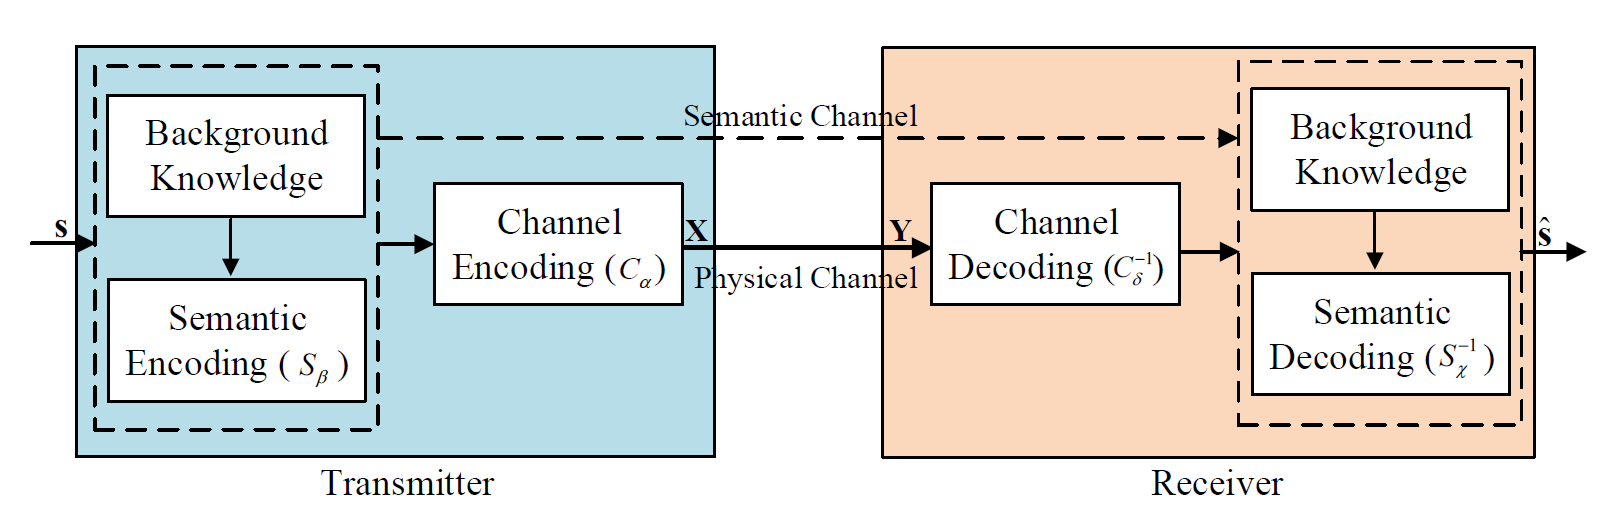
\includegraphics[width=0.6\linewidth]{figures/semcom}
		\caption{DeepSC --- модель семантической системы связи}
		\label{fig:semcom}
	\end{figure}
	
	На рисунке \ref{fig:semcom} приведена общая схема предложенной семантической системы связи. Передатчик преобразует текстовое предложение $\mathbf{s}$ в поток комплексных символов $\mathbf{x}$, далее эти символы передаются по физическому каналу связи. Приемник получает искаженные каналом символы $\mathbf{y}$ и на выходе совместного канального и семантического декодера получает оценку $\hat{\mathbf{s}}$ переданного предложения $\mathbf{s}$. 
	
	Входом модели является предложение $\mathbf{s} = \begin{pmatrix} w_1,\,...,\,w_L \end{pmatrix}$, состоящие из слов $w_i$, а $L$ --- максимальная длина входного предложения (все предложения дополняются до максимального специальными pad-словами, выбрано равным 32). Передатчик состоит из 2 частей: семантический кодер $S_\beta$ и канальный кодер $C_\alpha$, которые находят оптимальное в семантическом смысле представление предложения для передачи его по каналу ($\alpha$ и $\beta$ --- их обучаемые параметры):
	\begin{equation}
		\mathbf{x}=C_\alpha(S_\beta(\mathbf{s})), 
	\end{equation}
	где $\mathbf{x}\in \mathbb{C}^M$, то есть предложение передается с использованием $M$ комплексных символов (выбрано 8). В статье рассматривается простейшая модель беспроводного канала --- релеевский канал с временем когерентности $M$ (то есть канал остается неизменным во время передачи одного предложения):
	\begin{equation}
		\mathbf{y} = h \mathbf{x} + \mathbf{n},
	\end{equation}
	здесь $\mathbf{y}\in \mathbb{C}^M$ --- принятые символы, $h\sim \mathcal{CN}(0,\,1)$  --- комплексный коэффициент изменения амплитуды сигнала в канале соответствующий релеевскому каналу, и АБГШ  $\mathbf{n}\sim\mathcal{CN}(0,\,\sigma_n^2)$. Можно заметить, что данная модель канала дифференцируемая. Приемник последовательно применяет канальный $C_\delta^{-1}$ и семантический $S_\chi^{-1}$ декодеры ($\delta$ и $\chi$ --- их обучаемые параметры) и получает оценку $\hat{\mathbf{s}}$ переданного сообщения:
	\begin{equation}
		\hat{\mathbf{s}}=S_\chi^{-1}(C_\delta^{-1}(\mathbf{y})).
	\end{equation}
	
	В качестве функции потерь выбрана перекрестная энтропия между распределением слов в предложении на каждой позиции на передатчике $q(w_l)$ (one-hot векторы, так как известно, какие слова передавались) и оценкой распределения слов на приемнике $p(w_l)$:
	
	\begin{equation}
		\mathcal{L}_\text{CE}({\mathbf{s}},\,\hat{\mathbf{s}},\,\alpha,\,\beta,\,\chi,\,\delta) = 
		- \sum\limits_{l=1}^{L} q(w_l) \log(p(w_l)) + (1-q(w_l)) \log(1-p(w_l)).
	\end{equation}
	
	Так, при оптимизации данной функции потерь на большом корпусе текста, совместная система внешнего семантического и внутреннего канального кодеров и декодеров будет приближать распределение слов на приемнике к распределению на передатчике, это будет означать, что система обучилась извлекать и восстанавливать семантическую информацию из предложения. Также, выбор определенной направленности текстов при обучении может специализировать модель для передачи подобных текстов: приемник и передатчик будут иметь специализированную общую базу знаний. В отличие от обычной <<классической>> системы связи, канальных кодер здесь нацелен на сохранение семантической информации, а не всей информации, содержащейся в передаваемом сообщении (иными словами, не требуется передать без ошибок каждый бит).
	
	При проектировании системы связи важным является максимизация пропускной способности канала. А  пропускная способность канала --- это супремум взаимной информации $I(\mathbf{x},\,\mathbf{y})$ по распределению передаваемых символов $\mathbf{x}$ (а в совместной оптимизации передатчик может корректировать распределение). Взаимная информация между передаваемыми и принимаемыми символами определяется как расстояние Кульбака-Лейблера между маргинальными распределениями $\mathbf{x}$, $\mathbf{y}$ и их совместным распределением:
	 \begin{equation}
	 	I(\mathbf{x},\,\mathbf{y}) = D_\text{KL}(p({x}, {y})||p({x}) p({y}))
	 \end{equation}
	 Данная величина является интегралом по вероятностому пространству, кроме того, в рассматриваемой задаче распределения непрерывные. Поэтому напрямую в таком виде взаимная информация недифференцируема и не может использоваться в функции потерь. Однако существуют теорема \cite{belghazi2018mine}, доказывающая, что $I(\mathbf{x},\,\mathbf{y})$ представима в виде:
	 \begin{equation} 
	 	I(\mathbf{x},\,\mathbf{y}) = 
	 	\underset{T: \Omega \rightarrow R}{\sup}\mathbb{E}_{p(x,y)}[T] -
	 	\log(\mathbb{E}_{p(x)p(y)}[e^T]),
	 \end{equation}
	где супремум взят по всем таким функциям $T$, что математические ожидания конечны. Авторы предлагают использовать в качестве $T$ полносвязную нейросеть, обучая $T$ в схеме без учителя (так как требуются только $\mathbf{x}$ и $\mathbf{y}$) совместно со всей системой связи. Так, данная модель во будет приближаться к оценке взаимной информации снизу. Вводится 
	\begin{equation}
		\mathcal{L}_\text{MI}(\mathbf{x},\,\mathbf{y},\,\tau,\,\alpha,\,\beta) = \mathbb{E}_{p(x,y)}[f_\tau] -
		\log(\mathbb{E}_{p(x)p(y)}[e^{f_\tau}]),
	\end{equation}
	где $f_\tau$ --- полносвязная нейросеть, $\tau$ --- ее параметры. Матожидание вычисляется непосредственно по элементам каждого батча. Батч делится на две равные части: $\mathbf{x}_1$, $\mathbf{x}_2$ и  $\mathbf{y}_1$, $\mathbf{y}_2$, для вычисления совместного распределения используются $\mathbf{x}_1$ и $\mathbf{y}_1$ (непосредственно переданные и принятые символы), а для маргинального --- $\mathbf{x}_1$ и $\mathbf{y}_2$ (символы, не связанные друг с другом). В таком виде, со знаком минус и некоторым коэффициентом $\lambda\in[0;1]$, взаимная информация может быть использована в общей функции потерь:
	\begin{equation}
		\mathcal{L} = \mathcal{L}_\text{CE} - \lambda \mathcal{L}_\text{MI}.
	\end{equation}

	\begin{figure}[h!]
		\centering
		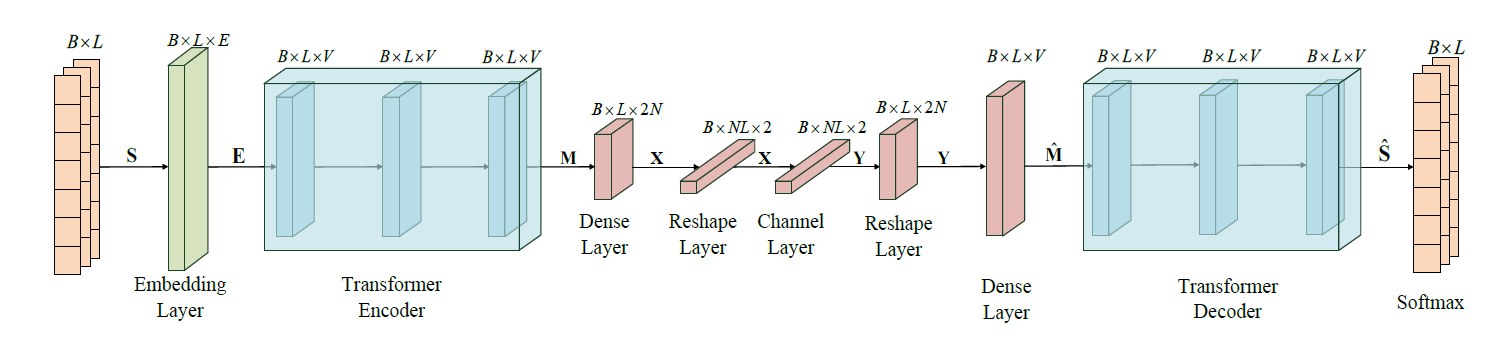
\includegraphics[width=0.8\linewidth]{figures/nn}
	\end{figure}
	\begin{figure}[h!]
		\centering
		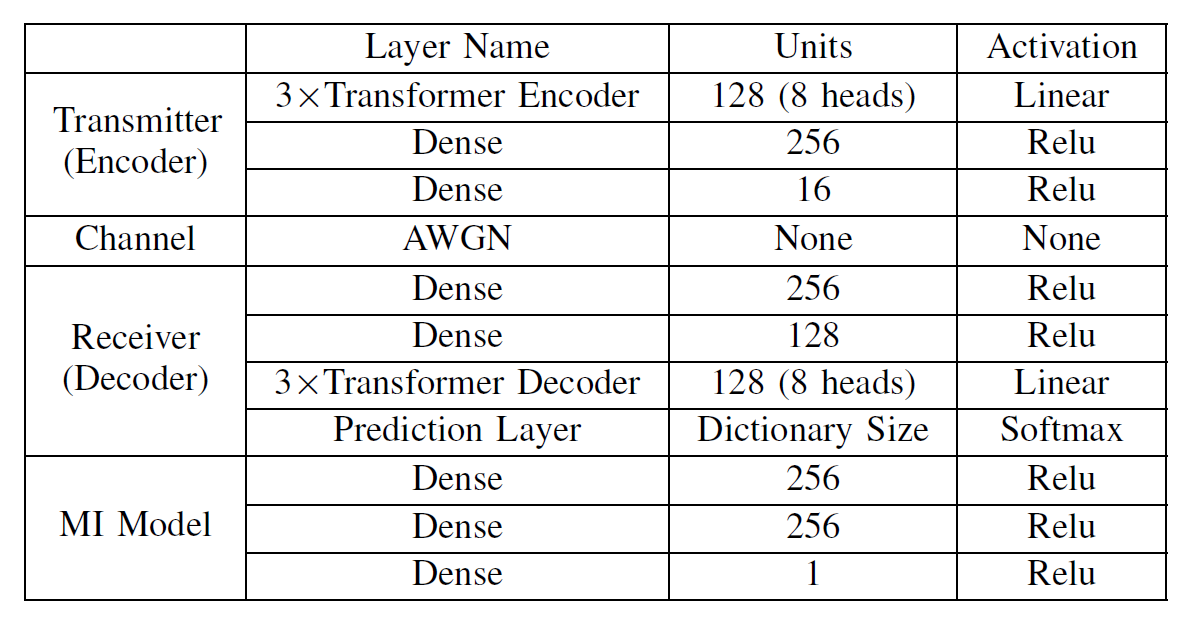
\includegraphics[width=0.4\linewidth]{figures/table}
		\caption{Архитектура модели семантической системы связи DeepSC}
		\label{fig:nn}
	\end{figure}
	
		
	Теперь в деталях опишем нейросетевые архитектуры всех элементов рассматриваемой семантической системы связи. Общая схема и таблица с параметрами приведена на рисунке \ref{fig:nn}. Семантический кодер состоит из трех слоев трансформеров (8-headed), канальный кодер состоит из двух слоев полносвязной нейросети. АБГШ канал является лишь простой линейной операцией прибавления случайного белого гауссового шума. Приемник устроен симметрично: канальный декодер на основе двухслойной полносвязной нейросети для обработки полученных символов и семантический декодер, состоящий из трех слоев трансформеров (8-headed), который оценивает полученные слова в предложении. Трансформер способен преобразовывать эмбеддинг отдельного слова на основе предыдущих слов в предложении (self-attention), то есть контекста, семантики слова. Последним слоем декодера является полносвязный слой и softmax, где для каждой позиции слова формируется распределение возможных токенов-слов в предложении. Здесь трансформер позволяет лучше предсказывать (декодировать по максимуму вероятности) очередное слово в предложении из его контекста.
	
	Псевдоалгоритм обучения модели представлен на рисунке \ref{fig:alg}   
	
	\begin{figure}[h!]
		\centering
		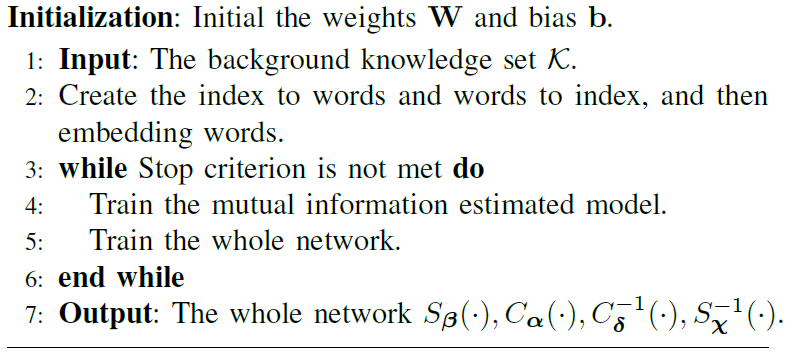
\includegraphics[width=0.4\linewidth]{figures/alg}
		\caption{Алгоритм обучения DeepSC}
		\label{fig:alg}
	\end{figure}
	
	\section*{Метрики и их критика}
	
	Рассмотрим используемые метрики оценки качества передачи текстовой информации. Используется BLEU (Bilingual Evaluation Understudy) \cite{papineli2002bleu}, классическая метрика для оценки качества перевода (здесь будет использована для оценки качества декодирования на приемника) и более интересная метрика --- косинусное расстояние между эмбеддигнами принятых и переданных предложений на основе предобученной модели BERT (Bidirectional Encoder Representations from Transformers) \cite{devlin2018bert}, авторы назвали последнюю метрику Sentence Similarity \cite{xie2021sem}. 
	
	Авторы утверждают, что первая метрика менее предпочтительна, так как основана на частотностях встречи $n-грамм$ из переданного сообщения в принятом, что не полностью оценивает семантику предложения: например, перефразирование или синонимы будут снижать метрику так же, как и замена на случайные слова.
	Однако и предложенная авторами метрика на основе предобученного BERT также нельзя считать удовлетворительной. BERT обучался на большом корпусе текстов, при этом можно естественно предположить, что в них содержалось очень ограниченное число ошибок, до и то не таких, которые характерны в передаче информации с битовыми ошибками, то есть когда могут возникнуть случайные замены одной буквы на другую. Кроме того, относительно высокие значения метрики могут быть даны предложению с абсолютно искаженным смыслом. 
	
	Рассмотрим предложение: <<Education is what remains after one has forgotten what one has learned in school>>. Его токенизация предложения BERT'ом будет иметь вид:  ['education',
	'is',
	'what',
	'remains',
	'after',
	'one',
	'has',
	'forgotten',
	'what',
	'one',
	'has',
	'learned',
	'in',
	'school']
	
	Во первых, Sentence Similarity крайне чувствительна к сдвигам между токенами. Например, при наличии ошибки в одной букве (а это может быть всего лишь одна битовая ошибка на все предложение) BERT использует другую токенизацию предложения. Так, для <<\textcolor{red}{Q}ducation is what remains after one has forgotten what one has learned in school>>, токенизация будет иметь вид: ['q',
	'\#\#du',
	'\#\#cation',
	'is',
	'what',
	'remains',
	'after',
	'one',
	'has',
	'forgotten',
	'what',
	'one',
	'has',
	'learned',
	'in',
	'school']. Это приведет к увеличению длины вектора токенов и сдвигу относительно исходного предложения, что значительно снижает величину метрики до 0.43. При этом едва ли смысловое содержание предложения хоть сколько нибудь поменялось. Более искаженный пример: <<Educafion is wzat rempins aftqr onx hay porgotten uhat kne has lehrned in school>>  с исходным предложением имеет крайне низкое Sentence Similarity равное 0.28, однако человек (да и дожным образом построенный алгоритм) легко сможет восстановить исходное сообщение.
	
	Во вторых, подбор синонимичных слов или согласованных по частям речи слов в некоторых позициях может несильно снизить метрику, при этом смысл сообщения абсолютно поменяется. Так, для абсурдного предложения, частично сохраняющего структуру исходного: <<Training is what remains before cat has remembered what nine has taught in kindergarten>> , значение Sentence Similarity равняется 0.62, что в почти полтора раза выше, чем для случая ошибки в одной букве. Заметим, что как раз значение такого порядка приводится в результатах экспериментов для самых низких SNR \cite{xie2021sem} (рисунок 7). 
	
	Таким образом, приводимые в статье \cite{xie2021sem} метрики нельзя считать удовлетворительными в контексте оценки качества системы связи, особенно при сравнении <<классических>> и семантических систем связи.
	
	
	\section*{Эксперимент}
	
	
	Как указывают сами авторы, результаты оптимизации сильно зависят от параметров оптимизационного алгоритма, кроме того, авторы не указали рекомендации по выбору параметра $\lambda$. Поэтому точное воспроизведение результатов затруднено. Однако все же можно качественно продемонстрировать результаты работы системы рассмотренной семантической связи. Я остановился на канале с АБГШ с коэффициентом при взаимной информации в функции потерь $\lambda = 0.0001$. 
	
	\begin{figure}[h!]
		\centering
		\begin{subfigure}{0.35\linewidth}
			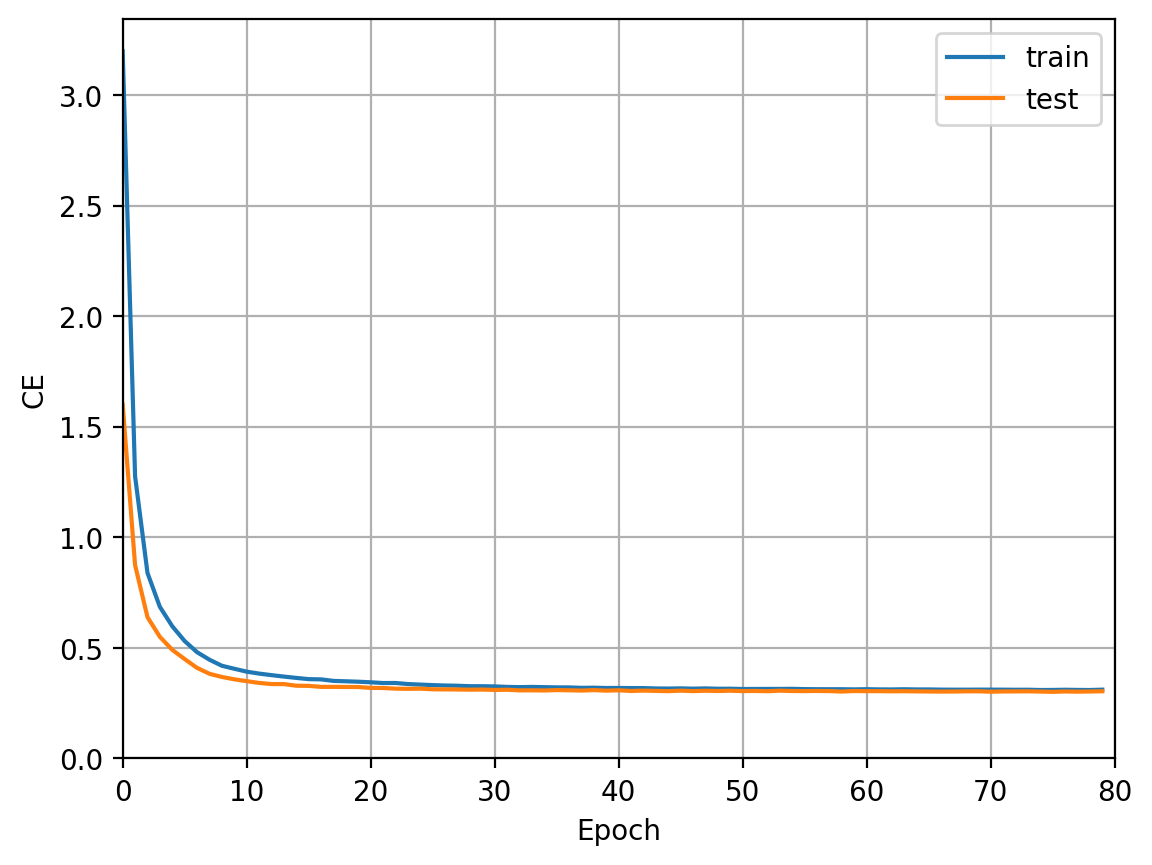
\includegraphics[width=\linewidth]{figures/ce}
		\end{subfigure}
		\begin{subfigure}{0.35\linewidth}
			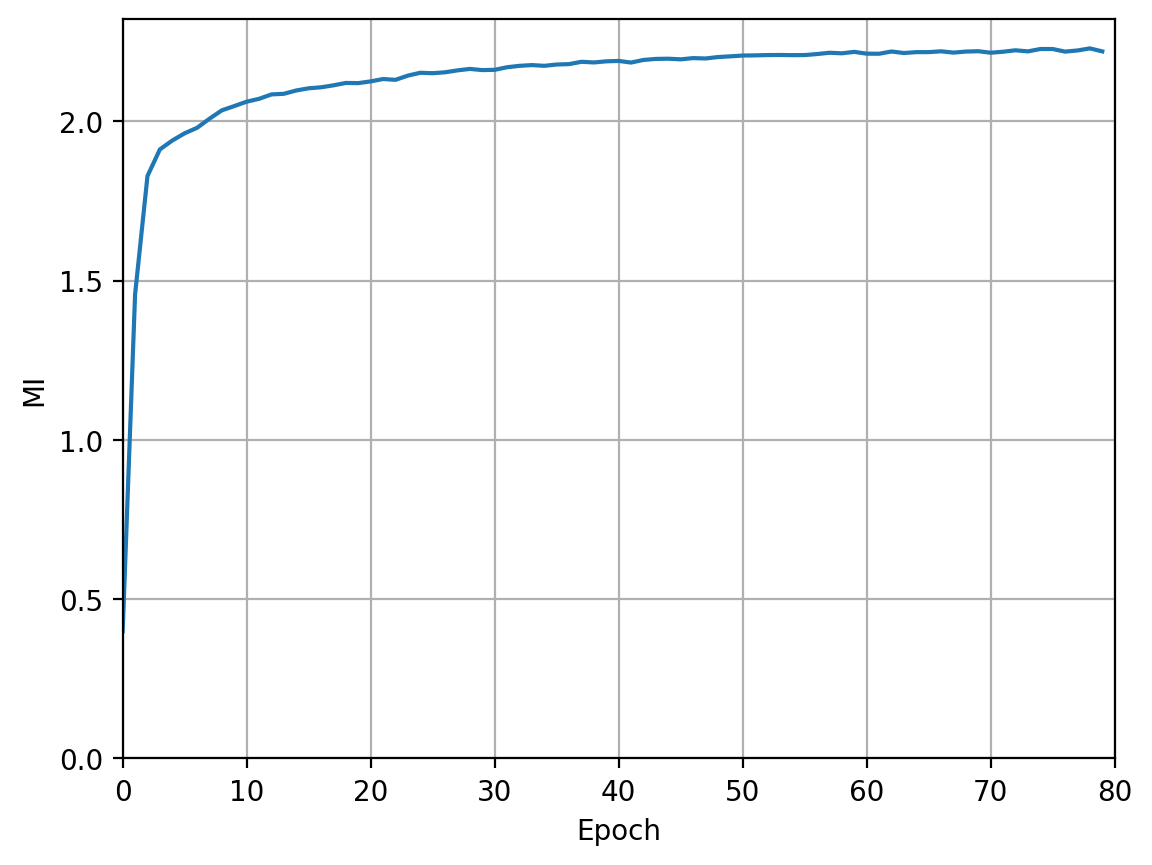
\includegraphics[width=\linewidth]{figures/mi}
		\end{subfigure}
		\caption{Обучение модели: перекрестная энтропия (слева) и взаимная информация (справа)}
	\end{figure}
	
	\begin{figure}[h!]
		\centering
		\begin{subfigure}{0.35\linewidth}
			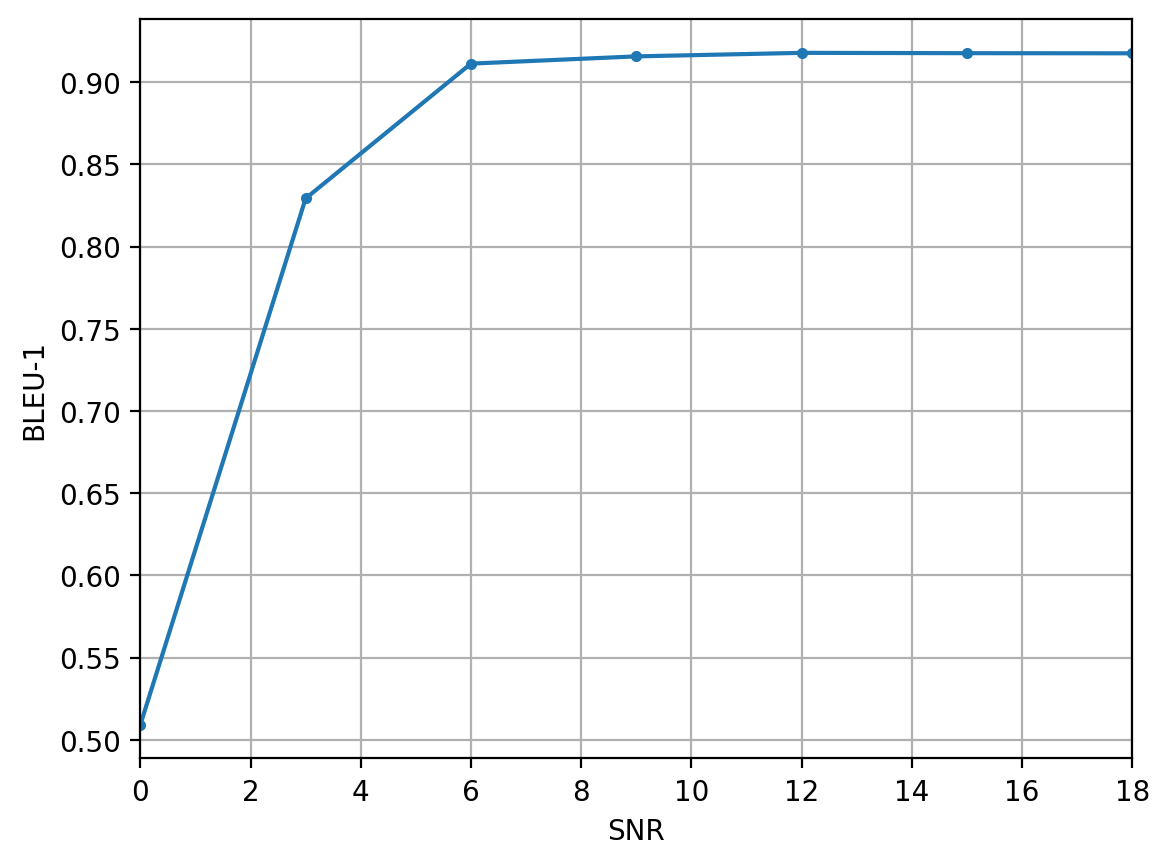
\includegraphics[width=\linewidth]{figures/bleu}
		\end{subfigure}
		\begin{subfigure}{0.35\linewidth}
			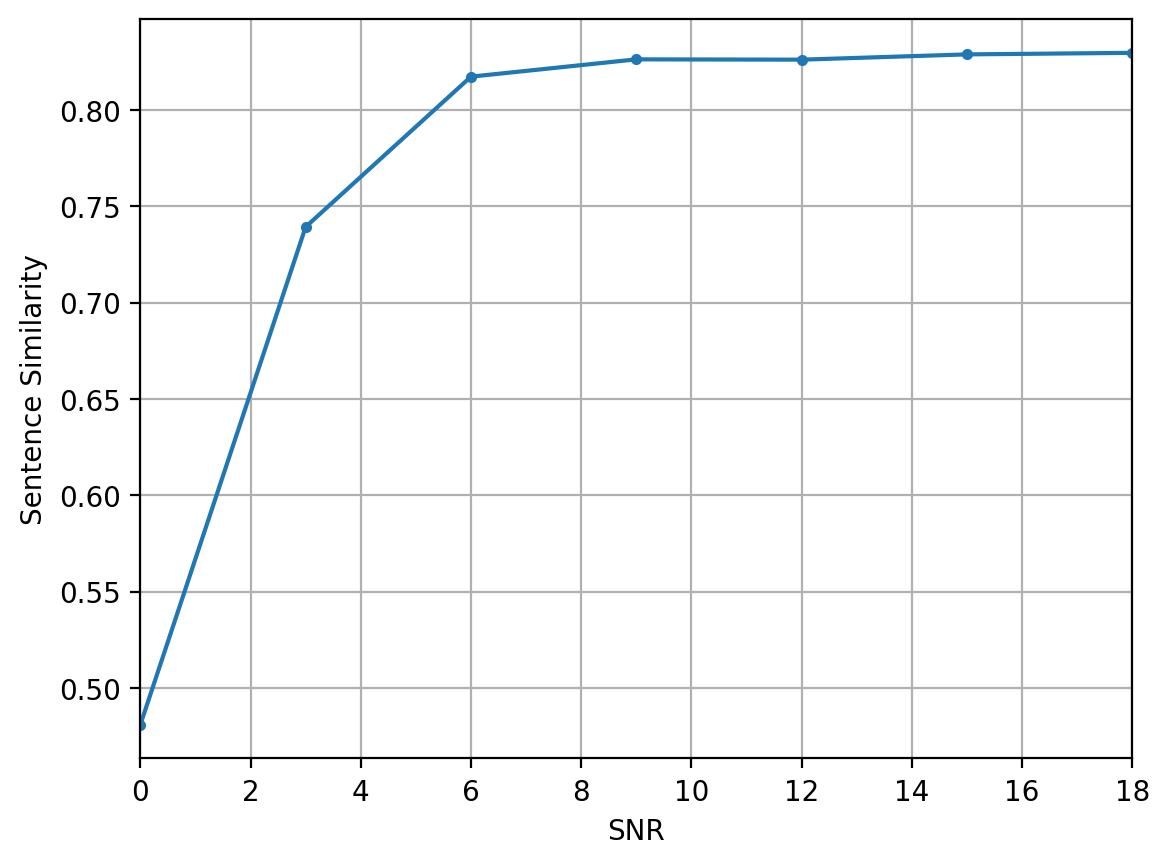
\includegraphics[width=\linewidth]{figures/sim}
		\end{subfigure}
		\caption{Метрики при различных SNR: BLEU-1 (слева) и Sentence Similarity (справа)}
	\end{figure}
	
	
	Как можно видеть, значение перекрестной энтропии уменьшается монотонно от эпохи к эпохе, переобучения не наблюдается. Взаимная информация монотонно растет и выходит на плато. Метрики BLEU-1 и Sentence Similarity ожидаемо растут при увеличении SNR, при низких SNR метрики в рассматриваемой системе семантической связи значительно превосходят <<классические>> (см. рисунок 6-7 \cite{xie2021sem}), но с важными оговорками, которые обсуждались в предыдущем разделе.
	
 	
	\section*{Выводы}
	В работе рассмотрена семантическая система связи на основе моделей глубокого обучения \cite{xie2021sem}, экспериментально продемонстрирована работа подобной системы. В работе также приводится критика используемых в статье метрик. Использование предложенных семантических метрик является спорным решением, так как в текстовой выборке, по которой обучается построение эмбеддингов токенов, практически отсутствуют ошибки, особенно характерные для битовых ошибок в передаче данных. Поэтому замена нескольких символов на случайные может значительно снизить семантические метрики, при этом для человека оно будет оставаться абсолютно понятным и сохраняющим смысл (в отличие, например, замены столицы одного государства на столицу другого или слова на его антоним). Поэтому требуется создание специальных моделей оценки и исправление подобных ошибок для более объективного сравнения <<классических>> и семантических систем связи. Например, это может быть что-то вроде лучевого поиска по ближайшим реально существующим словам для <<классических>> систем или же специальная модель трансформера, способная работать с данными, содержащими ошибки. 
	
	Тем не менее, введение семантической обработки информации в структуру систем связи обладает высоким потенциалом для стандартов связи будущих поколений в контексте оптимизации объема передаваемой информации, ее достоверности и полноты.

	\clearpage
	\newpage
	\begin{thebibliography}{0}
		\addcontentsline{toc}{section}{\refname}
		\bibitem{xie2021sem} Xie, Huiqiang \& Qin, Zhijin \& Li, Geoffrey and Juang, Biing-Hwang. Deep Learning Enabled Semantic Communication Systems (2021).
		
		\addcontentsline{toc}{section}{\refname}
		\bibitem{shannon1948comm} Shannon, Claude. A Mathematical Theory of Communication (1948)
		
		\addcontentsline{toc}{section}{\refname}
		\bibitem{weaver1949comm} Weaver, Warren \& Shannon, Claude. Recent contributions to the mathematical theory of communication (1949).
		
		\addcontentsline{toc}{section}{\refname}
		\bibitem{casella2002stat} Belghazi, Ishmael \& Rajeswar, Sai \& Baratin, Aristide \& Hjelm, R Devon and Courville, Aaron. MINE: Mutual Information Neural Estimation (2018). 
		
		\addcontentsline{toc}{section}{\refname}
		\bibitem{vaswani2017tr} Ashish Vaswani \& Noam Shazeer \& Niki Parmar \& Jakob Uszkoreit \& Llion Jones \& Aidan N. Gomez \& Lukasz Kaiser and Illia Polosukhin. Attention Is All You Need (2017) 		
		
		\addcontentsline{toc}{section}{\refname}
		\bibitem{papineli2002bleu} Papineni, K. \&  Roukos, S. \& Ward, T. and Zhu, W. J. BLEU: a method for automatic evaluation of machine translation (2002)
		
		\addcontentsline{toc}{section}{\refname}
		\bibitem{devlin2018bert} Jacob Devlin \& Ming-Wei Chang \& Kenton Lee and Kristina Toutanova. BERT: Pre-training of Deep Bidirectional Transformers for Language Understanding (2018)
		
		\addcontentsline{toc}{section}{\refname}
		\bibitem{belghazi2018mine} Belghazi, Ishmael \& Rajeswar, Sai \& Baratin, Aristide \& Hjelm, R Devon and Courville, Aaron. MINE: Mutual Information Neural Estimation (2018). 
		
		
		
	\end{thebibliography}
	
	
\end{document}